\begin{figure}[ht!]  % 'htbp' suggests placement options
    \centering
    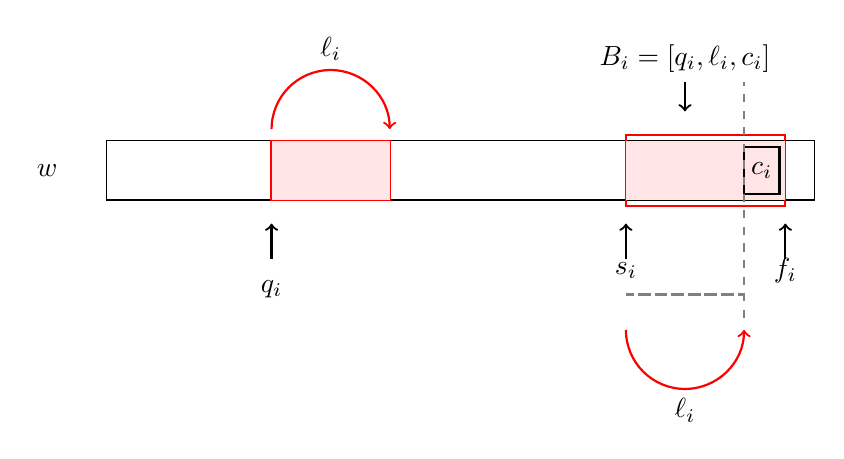
\begin{tikzpicture}[scale=1.5]
        % Main Rectangle w
        \draw (0,0) rectangle (6,0.5);
        \node at (-0.5, 0.25) {\(w\)};
        % Smaller Rectangle 1 - Border color red
        \draw[draw=red, thick] (1.4,0) rectangle (2.4,0.5);
        \draw[->, thick] (1.4,-0.5) -- (1.4,-0.2);
        \node[align=center, below] at (1.4,-0.6) {\(q_i\)};
        
        \fill[red!10] (1.4,0) rectangle (2.4,0.5);
        % Semicircular arrow
        \draw[->, thick, red] (1.4,0.6) arc[start angle=180, end angle=0, radius=0.5cm];
        \node[align=center, above] at (1.9,1.1) {\(\ell_i\)};
        
        % Smaller Rectangle 2 - Border color red
        \draw[draw=red, thick] (4.4,-0.05) rectangle (5.75,0.55);
        
        \fill[red!10] (4.4,0) rectangle (5.75,0.5);
        % Arrow and label for j
        \draw[->, thick] (4.9,1) -- (4.9,0.75);
        \node[align=center, above] at (4.9,1) {\(B_i=[q_i,\ell_i,c_i]\)};
        % Dibuja las flechas
        \draw[->, thick] (4.4,-0.5) -- (4.4,-0.2);
        \draw[->, thick] (5.75,-0.5) -- (5.75,-0.2);

        % Añade las etiquetas s_i y f_i cerca de las flechas
        \node at (4.4,-0.6) {$s_i$};
        \node at (5.75,-0.6) {$f_i$};

            % Draw an inverted elliptical arc
        \draw[->, thick, red] (4.4, -1.1) arc[start angle=180, end angle=360, x radius=0.5cm, y radius=0.5cm];
    
        % Label below the arc
        \node[align=center, below] at (4.9,-1.6) {$\ell_i$};
    
        % Smaller Rectangle 3 - Border color c_i
        \draw[draw=black, thick] (5.4,0.05) rectangle (5.7,0.45);
         % Draw a vertical dashed line at x = 4.4
        \draw[gray, thick, dashed] (5.4, -1) -- (5.4, 1); % Define suitable y-coordinates for your needs
        \draw[draw=gray, thick, dashed] (4.4,-0.8) rectangle (5.4,-0.8);
        % Añade la etiqueta c_i en el centro del rectángulo
        \node at (5.55,0.25) {$c_i$};
        
        
    \end{tikzpicture}
    \caption{An Illustration of constructing the $i$-Block.}
    \label{fig:compressionBlockWorking}
\end{figure}